\documentclass[10pt, a4paper]{article}

% \usepackage{fullpage}

\usepackage[margin=1in]{geometry}
% \usepackage[top=1in, bottom=1in, left=0.5in, right=0.5in, paperwidth=5in, paperheight=7in]{geometry}

% \usepackage{amsfonts}
\usepackage{amsfonts, amssymb, amsmath}

\usepackage{tikz,pgfplots}

\usepackage{graphicx}

\usepackage{float}





\def\equation1{y=\dfrac{x}{3x^2+x+1}}

\newcommand{\set[1]}{\setlength\itemsep{#1em}}




\newcommand\calculator{\tikz{
		\node (c) [inner sep=0pt, draw, fill=black, anchor=south west]{\phantom{N}};
		\begin{scope}[x=(c.south east),y=(c.north west)]    \fill[white] (.1,.7) rectangle (.9,.9);    
		\foreach \x in {.1, .33, .55, .79}{    
		\foreach \y in {.1, .24, .38, .53}{    
		\fill[white] (\x,\y) rectangle +(.11,.07);}} 
		\end{scope} }}
		\def\calcicon#1{\noindent#1 \calculator\ }



\begin{document}

packages\\


in the documentclass we can mention "a4paper" or "letterpaper" to specify the paper size\\

we can also use a percent sign in front of a line to comment it out\\

packages can be included in the preamble\\
preamble is the place which is in-between the documentclass and begin document\\
we can give some options when we load a package\\
options can be given in square brackets before the name of the package in braces\\
if we are not giving any options then multiple packages can be specified in a single statement by giving comma\\


the package "fullpage" is used for giving 1 inch margins on all sides of all pages\\
otherwise by default there is a lot of space used up by the margins, margins are too large by default\\

the package "geometry" is used to explicitely specify the margin size\\
if we use this then we do not need the "fullpage" package\\
we can specify the margins in inches or centimeters\\
we can also adjust the papersize\\

the package "amsfonts" allows us to use some specialized math notation\\
also this will give us hints for the available notation commands while we type\\

\begin{enumerate}

\item This is the symbol for all real numbers: $\mathbb{R}$.
\item This is the symbol for the set of integers: $\mathbb{Z}$.
\item This is the symbol for the set of rational numbers: $\mathbb{Q}$.

\end{enumerate}


macros\\


you can also load some macros in your preamble\\
macros are used to define your own custom latex commands\\

\begin{enumerate}

\set[3]

\item Lets examine the function $\equation1$ \\
here we have defined a macro by the name as "equation1"\\
and added the equation as body of it\\
so anywhere in the document we can use the macro \\

\item again we are looking at the equation $\equation1$ \\

\item we have also defined a new command called "set" as a macro\\
this is like a function\\
where function name is "set" and inside brackets we are accepting a parameter\\
and using that parameter within the body of the function where we have written "hash 1"\\
so this is a dynamic macro which will make changes according to the parameter that we pass\\
here in this case we are defining the space between each of the list items\\

\item \calculator\ again we are looking at the equation $\equation1$ \\
here we are adding a calculator symbol at the beginning with a space after that indicated by the closing backslash after the calculator\\
for this we have included the packages "tikz" and "pgfplots"\\

\end{enumerate}



inserting graphics (image files) \\


save the image files in the same folder as the tex file\\
we also need the package "graphicx" for inserting images\\
we have to specify the name of the file without the extension\\
and also the scale ie the size of the image on a scale of 0 to 1\\

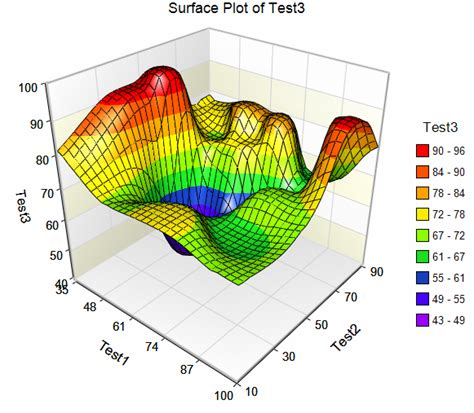
\includegraphics[scale=0.5]{plot1}

we can also specify the height and width of the image\\


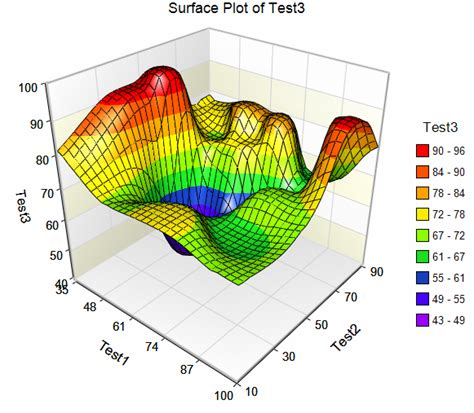
\includegraphics[width=3.5in, height=5in]{plot1}


we can use inches, centimeters, or percent\\
below we are making the image 0.5 ie half of the text width\\
not page width which includes the margins\\

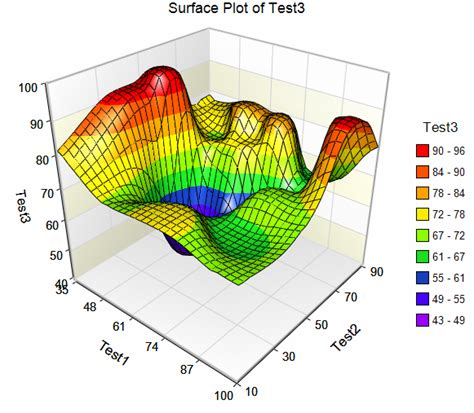
\includegraphics[width=0.5\textwidth]{plot1}


to make the image centered\\
\begin{center}
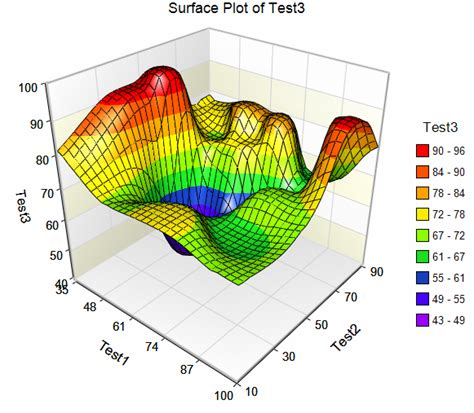
\includegraphics[width=0.5\textwidth]{plot1}
\end{center}


to place the image precisely use "figure" \\
in it use "h" to specify to place it "here"\\
in it use "t" to specify to place it in the "top" of the page\\
in it use "b" to specify to place it in the "bottom" of the page\\
in it use capital "H" to specify to place it in right here where it is coded, but that requires the package "float", this is also used to place tables, not just images\\
\begin{figure}[h]
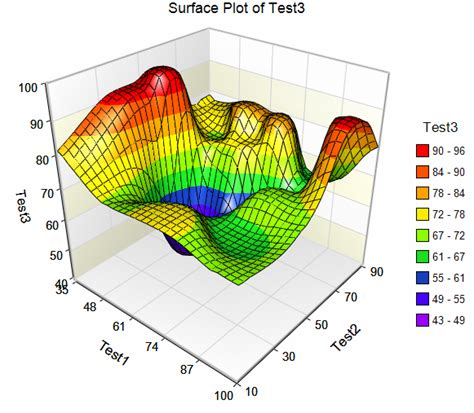
\includegraphics[width=0.4\textwidth]{plot1}
\end{figure}


we can also center the image with "centering" along with figure\\
we can also add a caption below the image by using "caption"\\
this automatically labels the caption as "Figure 1:"
\begin{figure}[h]
\centering
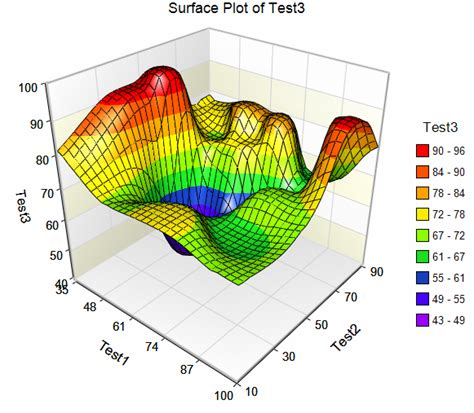
\includegraphics[width=0.4\textwidth]{plot1}
\caption{This is a plot}
\end{figure}



NOTE:\\
we can add a "backslash comma" to manually add a space somewhere inside a text\\
the compiler ignores all         extra spaces\\
like spaces \,\,\,\,\,\,\,\,\, in this line\\




\end{document}
